%
% teil3.tex -- Beispiel-File für Teil 3
%
% (c) 2020 Prof Dr Andreas Müller, Hochschule Rapperswil
%
\section{Fraktale Bildkomprimierung
\label{ifs:section:teil3}}
\rhead{Fraktale Bildkomprimierung}
Mit dem Prinzip dieser IFS ist es auch möglich Bilder zu Komprimieren.
Diese Idee hatte der Mathematiker Michael Barnsley, welcher mit seinem Buch Fractals Everywhere einen wichtigen Beitrag zum Verständnis von Fraktalen geliefert hat.
Das Ziel ist es ein IFS zu finden, welches das Bild als Attraktor hat.
In diesem Unterkapitel wollen wir eine Methode dafür anschauen.\cite{ifs:Rousseau2012}


Bis jetzt wurde in Zusammenhang mit IFS immer erwähnt, dass die Transformationen auf die ganze Menge angewendet werden.
Dies muss jedoch nicht so sein. 
Es gibt auch einen Attraktor, wenn die Transformationen nur Teile der Menge auf die ganze Menge abbilden.
Diese Eigenschaft wollen wir uns in der Fraktalen Bildkompression zunutze machen.
Sie ermöglicht uns Ähnlichkeiten zwischen kleineren Teilen des Bildes zunutze machen.
Es ist wohl nicht falsch zu sagen, dass Ähnlichkeiten zur gesamten Menge, wie wir sie zum Beispiel beim Barnsley Farn gesehen haben, bei Bilder aus dem Alltag eher selten anzutreffen sind.
Doch wie Finden wir die richtigen Affinen Transformationen, welche als IFS das Bild als Attraktor haben?

\subsection{das Kompressionsverfahren
\label{ifs:subsection:malorum}}
In der Beschreibung des Verfahrens wird sich auf Graustufenbilder bezogen. Wie das Verfahren für Farbbilder verwendet werden kann, wird später erläutert.

In einem ersten Schritt teilen wir das Bild in disjunkte benachbarte $b \times b$ Pixel-Quadrate auf. Diese Blöcke nennen wir Range-Blöcke der Menge $R=\{R_0,R_1,...R_m\}$
Im nächsten Schritt teilen wir das Bild in alle möglichen $2b \times 2b$ Pixel-Quadrate auf. Diese sind die Domain-Blöcke der Menge $D = \{D_0,D_1,...D_n\}$. 
Im dritten und letzten Schritt wird für jeden Range-Block $R_i$ ein Domain-Block $D_j$ gesucht, welcher ihm am ähnlichsten ist.

\subsubsection{Finden des ähnlichsten $D_j$}
Zuerst brauchen wir die Transformation um ein Element aus $D$ auf ein Element von $R$ Abzubilden.
\begin{align*}
	T(x,y,z) = 
	\begin{pmatrix}
		a & b & 0 \\
		c & d & 0 \\
		0 & 0 & s
	\end{pmatrix}
	\begin{pmatrix}
		x \\
		y \\
		z
	\end{pmatrix}
	+
	\begin{pmatrix}
		\alpha \\
		\beta \\
		g
	\end{pmatrix}
\end{align*}
Diese Transformation bildet den Pixel $P$ auf Koordinate $(x,y)$ und Graustufe $z$ auf den Pixel $P'$ ab.

Da wir mit Pixeln arbeiten, sind die Transformationen in der Ebene Beschränkt.
Diese wird durch die Parameter $a,b,c$ und $d$ bestimmt.
Mögliche Transformationen sind auf folgende Liste Beschränkt:
\begin{itemize}
	\item Identische Transformation, keine Änderung
	\item Drehung um 90, 180 oder 270 Grad.
	\item Spiegelung an der vertikalen, horizontalen und den Diagonalachsen.
\end{itemize}
$\alpha$ und $\beta$ verschieben den Pixel an die richtige Stelle.
Da wir ein $2b \times 2b$ Feld auf ein $b \times b$ Feld abbilden möchten, müssen wir zuerst $G_j$ um $1/2$ skalieren.
Dies erreichen wir, indem wir alle disjunkten $2 \times 2$ px Blöcke mit einem Pixel des Grautones deren Mittelwertes ersetzen.
Skaliert und transformiert erhalten wir $\tilde{D_j}$

Die Parameter $s$ und $g$ beschreiben die Änderung des Grautones. $s$ verändert den Kontrast und $g$ verschiebt die Töne auf die richtige Helligkeit. 
$s$ und $g$ werden mit der linearen Regression ermittelt. 
\begin{align*}
	z' = sz + g \\
	f(\tilde{D_j}) \text{, Funktion um das Bild eins Blockes zu erhalten}  \\
	s = \frac{cov(f(R_i), f(\tilde{D_j}))}{var(\tilde{D_j})} \\
	g = E(f(R_i)) - s E(f(\tilde{D_j}))
\end{align*}
Mit diesen Parametern haben wir nun die Transformation vollständig bestimmt.
Um zu beurteilen ob der Domain-Block $D_j$ mit der gefundenen Transformation $T$ dem Range-Block $R_i$ genügend ähnlich ist, berechnet man den quadratischen Abstand $e$.
\begin{align*}
	e = d(f(R_i), f(T(D_j)))
\end{align*}
Dieser Abstand sollte so klein wie möglich sein.
Die beste Kombination von $D_j$ und $T_i$ ist also diese, welche den kleinsten Abstand zum Block $R_i$ hat, und somit am ähnlichsten ist.

Am Ende des Verfahrens haben wir also für jeden $R_i$ einen passenden $D_i$ mit der zugehörigen Abbildung $T_i$ gefunden.

\subsubsection{Rekonstruktion des Bildes}
Mit den Gefundenen Abbildungen lässt sich das Bild generieren.
Wir beginnen wie schon im letzten Kapitel mit einer beliebigen Startmenge.
In unserem Fall ist dieses ein Bild  $f_0$ derselben Grösse.
Nun ersetzen wir jedes $R_i$ mit der Transformierten des zugehörigen Domain-Blocks $T(G_j)$.
Dies wird verkürzt als Operator $W$ geschrieben.
So erhalten wir ein neues Bild $f_1 = W(f_0)$.
Dieses Vorgehen führen wir iteriert aus bis wir von $f_n = W(f_{n-1})$ zu $f_{n-1}$ kaum mehr einen unterschied feststellen. Die Iteration hat nun ihren Fixpunkt, das Bild, erreicht.

\subsubsection{Farbbilder}
Dieses Verfahren mit Graustufenbilder lässt sich ganz einfach auf Farbbilder erweitern.
Jeder Pixel eines Farbbildes besteht aus einem Rot, Grün und Blauwert (RGB).
Teilt man ein Bild in die drei Farbkanäle auf, das heisst, es wird nur noch ein Farbwert benutzt, erhält man drei Bilder, welche wie ein Graustufenbild sind.
Nun wendet man auf jeden dieser Farbkanalbilder den Algorithmus an, und fügt nach der Rekonstruktion die Kanäle wieder zusammen. 

\subsubsection{Performance des Verfahren}
Dieser Grundalgorithmus der Fraktalen Bildkompression ist offensichtlich recht langsam und skaliert auch schlecht mit grösseren Bilder.
Man kann die Laufzeit zwar verbessern indem man die Domain-Blöcke auch disjunkt macht, und für weniger detailreiche Bilder ein grösseres $b$ wählt, jedoch wird er auch so nie so schnell wie zum Beispiel das jpeg verfahren.

\subsection{Beispiel}
Kommen wir nun zu einem Beispiel.
Wir Verwenden dafür den oben beschriebenen Algorithmus.
Die Range-Blöcke wurden $4\times4$ gewählt und die Dommain dementsprechend $8\times8$.
Um etwas Zeit bei der Komprimierung zu ersparen, wurden nur disjunkte Domain-Blöcke gebraucht.
Als erstes Beispiel wählen wir das 360x360px Bild von Rapperswil in Abbildung \ref{ifs:original}.
Der Algorithmus liefert uns für jeden Range-Block die benötigten Parameter.
Mit diesen lässt sich das Bild im Anschluss wieder Rekonstruieren.

Als Startbild wird ein mittelgraues 360x360px Bild gewählt, Abbildung \ref{ifs:bild0}.
Nun lassen wir das IFS laufen.
Wie wir in Abbildung \ref{ifs:rappirecoa} sehen, ist schon nach der ersten Iteration das Bild schon erkennbar.
Nach der fünften Iteration , Abbildung \ref{ifs:rappirecoc} gibt es fast keinen Unterschied mehr zur letzten Iteration, wir können die Rekonstruktion beenden.
\begin{figure}	
	\centering
	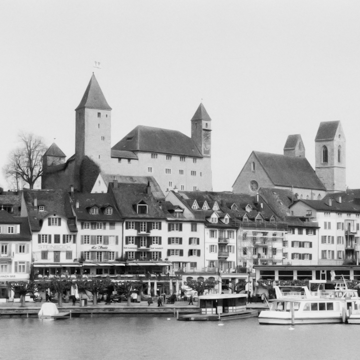
\includegraphics[width=0.4\textwidth]{papers/ifs/images/original}
	\caption{Original Bild von Rapperswil}
	\label{ifs:original}
\end{figure}
\begin{figure}
	\centering
	
\includegraphics[width=0.4\textwidth]{papers/ifs/images/rapperswil}
	\caption{Startbild}
	\label{ifs:bild0}
\end{figure}

\begin{figure}
	\centering
	\subfigure[]{
		\label{ifs:rappirecoa}
		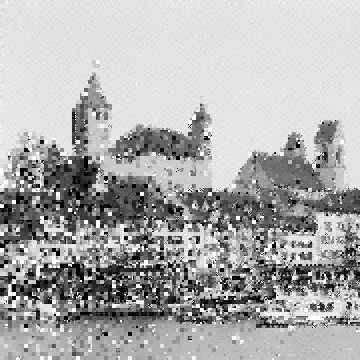
\includegraphics[width=0.32\textwidth]{papers/ifs/images/rapperswil01}}
	\subfigure[]{
		\label{ifs:rappirecob}
		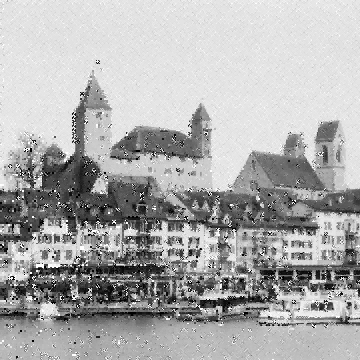
\includegraphics[width=0.32\textwidth]{papers/ifs/images/rapperswil001}} 
	\subfigure[]{
		\label{ifs:rappirecoc}
		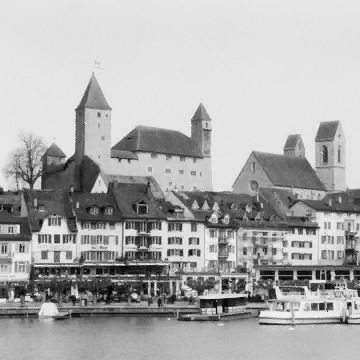
\includegraphics[width=0.32\textwidth]{papers/ifs/images/rapperswil04}}
	\caption{(a) 1. Iteration (b) 2. Iteration (c) 5. Iteration}
		\label{ifs:rappireco}
\end{figure}
